\newpage
\subsection{Sensoren auf dem Satellit}\label{sec:sensoraufcube}

\subsubsection{EDU}\label{edu}
Die Programmierung des EDU (Educational Module), welches sich im Cubesat der TU-Wien befindet, dient als eine Plattform, welche für Schülerinnen und Schüler zur Verfügung steht, um über ihre Software verschiedene Experimente durchzuführen. Das Modul besteht aus einem Raspberry PI, verschiedenen Sensoren und zwei Kameras (siehe Abb.), welche beide genutzt werden können. Die Ansteuerung der Sensoren funktioniert über den I2C-Bus. \\
\vspace{4mm}
\begin{figure}[H]
    \centering
    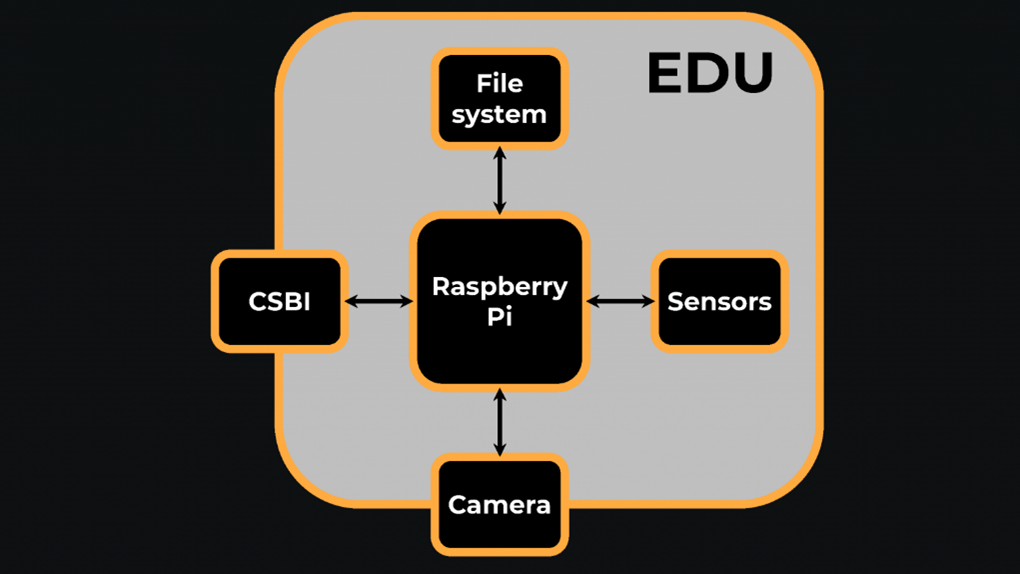
\includegraphics[scale = 0.8]{image/blockschaltnildedu.png}
    \caption{Blogschaltbild des EDUs}
    \label{fig:enter-label}
\end{figure}
\vspace{1mm}
Das System kann von jeder Person zuhause getestet werden. Dazu dient der EDU-Hat, eine Platine, welche die Sensorik des EDUs enthält und sich einfach auf einen Raspberry PI stecken lässt.
\newpage
\subsubsection{Sensorik des EDUs}
Auf dem EDU sind folgende Sensoren zu finden: 
\begin{itemize}
    \item Temperatursensor 
    \item Magnetfeldsenso
    \item Beschleunigungssensor
    \item Gyroskop
    \item GNSS-Empfänger
    \item UV-Sensoren
    \item Dosimeter
\end{itemize}
Der verwendete EDU-HAT (Simulation des EDUs für Selbstexperimente auf dem Boden) besitzt jedoch nur einen Temperatursensor, einen Beschleunigungssensor, einen Magnetfeldsensor, einen UV-Sensor und einen Gas Sensor. Die Montage einer Raspberry PI Kamera ist jedoch auch möglich.\\

\subsubsection{Temperatursensor}\label{temperatur}
Sowohl auf dem EDU-Hat als auch auf dem EDU selbst befinden sich 2 Sensoren, welche Temperaturen messen können. \\
\vspace{3mm}
Der Sensor TMP112\autocite{TMP112} ist ein rein digitaler Temperatursensor, welcher im Bereich von -40°C bis 125°C akkurat (±0,5°C bei 0° bis 65°C und ±1°C bei -40 bis 125°C) Temperaturen messen kann. Die Betriebsspannung des Sensors liegt bei 1.4V-3.3V bei einem maximalen Strom von 10µA. \\
\vspace{3mm}
Der Gas Sensor BME688\autocite{BME688} dient als Feuchtigkeitssensor, Gassensor und als guter Temperatursensor. Auch ist die Messung des Luftdrucks möglich. Die Betriebsspannung des Sensors liegt zwischen 1.71V-3.6V, während der Sensor je nach Betriebsmodus zwischen 2,1µA und bis zu 0,9mA Strom verbraucht. Der Arbeitsbereich des Sensors liegt zwischen -40°C bis 85°C für die Temperatur, 0-100°C für Luftfeuchtigkeit und Gaserkennung und 300-1100 hPa für den Luftdruck. 

\subsubsection{Magnetfeldsensor/Gyroskop}\label{magentsen}
Der BMM150\autocite{BMM150} ist ein dreiachsiger geomagnetischer Sensor, welcher sich für die Messung von Magnetfeldern und deren Einwirkungen eignet. Der Arbeitsbereich des Sensors liegt zwischen -40°C bis +85°C bei einer Betriebsspannung von 1.62V-3.6V. Auch der Stromverbrauch ist bei 170µA minimal. Die Rückgabe des Sensors besteht aus X, Y und Z Werten, welche die Stärke des Magnetfeldes in den verschiedenen Richtungen darstellen. 

\subsubsection{Beschleunigungssensor}\label{beschleuni}
Der Beschleunigungssensor ADXL345\autocite{ADXL345} dient als dynamischer Sensor, indem er Bewegung und Schock in G-Kräften zurückgibt. Der wichtigere Messbereich des ADXL345 Sensors ist die statische Messung, welche die Gravitation auf den verschiedenen Achsen zurückgibt. Aus dieser Information heraus kann der Winkel des Sensors ausgerechnet werden und somit als Gyroskop Sensor verwendet werden. \\
\vspace{3mm}
Der Stromverbrauch des Sensors liegt bei 40µA bei einer Betriebsspannung von 2.0V bis 3.6V. Der Sensor hat eine Auflösung von 13-Bit und misst in den Bereichen von ±16g, was umgerechnet rund ±156,91 m/s² entspricht. \\
\vspace{3mm}
Die Rückgabewerte des Beschleunigungsmessers entsprechen den G-Kräften an den X, Y- und Z-Achsen.

\subsubsection{UV-Sensor}\label{uvsens}
Der UV-Sensor GUVA\_C32 dient zur Messung von UV-Strahlen welche sich im Orbit, bzw. auf dem Boden befinden. UV-Strahlungen werden in Stärkegraden\autocite{Cosmic} als UV-Index (1-14 UV) angegeben. Die Betriebsspannung des Sensors liegt zwischen 2.6V bis 3.6V bei einem Stromverbrauch von 100µA.  

\subsubsection{Dosimeter}\label{dosimet}
Der Dosimeter ist einer der Sensoren, welche auf der EDU-Hat nicht vorhanden sind. Seine Aufgabe ist es ionisierte Strahlung zu empfangen. Strahlungen dieser Art sind hauptsächlich in höheren Elevationen verbreitet (siehe Abb. 40).\\
\vspace{3mm}
\begin{figure}[H]
    \centering
    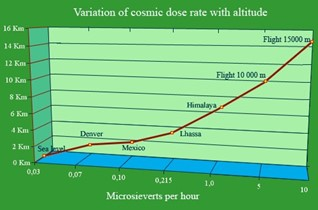
\includegraphics[scale=1.2]{image/bilduv.jpg}
    \caption{Korrelation Dosimeter}
    \label{fig:enter-label}
\end{figure}
Abbildung 40: Zu sehen ist die Korrelation zwischen der Elevation und des Mikrosieverts pro Stunde. Mikrosieverts beschreibt hierbei das stochastische Gesundheitsrisiko, welches durch ionisierte Strahlung verursacht wird.


